\documentclass{article}[18pt]
\usepackage{../../../../format}
\lhead{A Level Maths - FP2}

\begin{document}
\begin{center}
\underline{\huge First Order Differential Equations}
\end{center}
\section{Families of curves}
General solutions with a constant of integration C will give rise to a family of curves.\\
\\
If given boundary conditions we can find specific solutions.
\subsection{Example}
Find the solution to:\\
\\
$\dfrac{dy}{dx}=2$\\
\\
$y=2x+c$\\
\\

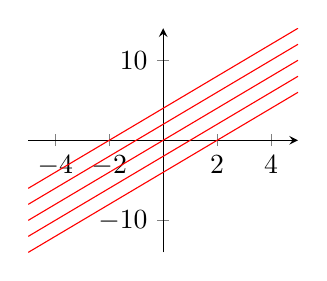
\begin{tikzpicture}
\begin{axis}[axis lines=middle,scale=0.5]
\addplot[color=red]{2*x};
\addplot[color=red]{2*x+2};
\addplot[color=red]{2*x+4};
\addplot[color=red]{2*x-2};
\addplot[color=red]{2*x-4};
\end{axis}
\end{tikzpicture}
\section{Introduction to first order differential equations}
Implicitly differentiate:\\
$x^3y \quad \textrm{wrt}x$\\
$3x^2y+x^3\dfrac{dy}{dx}$\\
\\
We can use this method in reverse to solve first order DEs
\subsection{Example 1}
$$x^3\dfrac{dy}{dx}+3x^2y=\sin(x)$$
\textcolor{red}{We look for standard patterns in the LHS and look to rewrite using the reverse implicit product rule}\\
$$\frac{d}{dx}(x^3y)=\sin(x)$$
$$x^3y=-\cos(x)+c$$
$$y=\frac{-\cos(x)+c}{x^3}$$
\textcolor{red}{If given an (x,y) point a particular solution can be found}\\
\\
In general:
$$\mathlarger{f(x)\frac{dy}{dx}+f'(x)y=\frac{d}{dx}(f(x)y)}$$
\newpage
\section{Solving first order DE using an integrating factor}
Solving $\dfrac{dy}{dx}+P(x)y=Q(x)$\\
\\
IF(Integrating factor) is found by finding $\mathlarger{e^{\int p(x) \ dx}}$ And multiplying the DE by the IF.\\
\\
This will result in the DE being in the form:
$$f(x)\frac{dy}{dx}+f'(x)y$$
This form can then be shortened by integrating:
$$\int f'(x)g(x)+f(x)g'(x) dx=f(x)g(x)+c$$
Integrate both sides then simplify
\subsection{Example}
$$p\frac{dx}{dt}+qx=r \qquad \textrm{Where p,q and r are constants}$$
\textit{Given that $x=0$ when $t=0$}\\
\textit{Find x in terms of t}\\
\\
\textcolor{red}{Divide through by p to ensure $\frac{dx}{dt}$ has no multiplier}
$$\frac{dx}{dt}+\frac{q}{p}x=\frac{r}{p}$$
\textcolor{red}{Find the integrating factor (IF)}
{\Large
$$IF: \mathlarger{e^{\int \frac{q}{p} \ dt}=e^\frac{qt}{p}}$$}
\textcolor{red}{Multiply through by the IF to make the equation in the right form}
{\Large
$$e^\frac{qt}{p}\frac{dx}{dt}+\frac{q}{t}xe^\frac{qt}{p}=\frac{r}{p}e^\frac{qt}{p}$$}
\textcolor{red}{Integrate both sides, simplify the LHS}
{\Large
$$xe^\frac{qt}{p}=\int \frac{r}{p}e^\frac{qt}{p} \ dt$$}
\textcolor{red}{Do the integration on the RHS and simplify}
{\Large
$$xe^\frac{qt}{p}=\frac{r}{q}e^\frac{qt}{p}+c$$}
\textcolor{red}{Substitute in x=0 and t=0 to find the value of c}
$$0=\frac{r}{q}+c$$
$$c=-\frac{r}{q}$$
\textcolor{red}{Substitute in the value of c and divide through by the IF}
{\Large
$$xe^\frac{qt}{p}=\frac{r}{q}e^\frac{qt}{p}-\frac{r}{q}$$
$$x=\frac{r}{q}-\frac{r}{q}e^{-\frac{qt}{p}}$$}
\section{First order DE with given substitution}
\textbf{Type 1} reduces to separation of variables\\
\\
\textbf{Type 2} reduces to $\dfrac{d}{dx}(f(x)y)$ form\\
\subsection{Type 1}
\textit{Show that the substitution $z=\dfrac{y}{x}$ transforms}
$$(1)\quad \frac{dy}{dx}=\frac{x^2+3y^2}{2xy}$$
\begin{center}
to
\end{center}
$$(2)\quad x\frac{dz}{dx}=\frac{1+z^2}{2z}$$
\textcolor{red}{We need to find $\frac{dz}{dx}$ and replace y in (1)}\\
$$y=xz \quad \quad \frac{dy}{dx}=z+x\frac{dz}{dx}$$
$$x\frac{dz}{dx}=\frac{x^2+3(xz)^2}{2x(xz)}-z$$
$$x\frac{dz}{dx}=\frac{1+3z^2}{2z}-z$$
$$x\frac{dz}{dx}=\frac{1+z^2}{2z}$$
\textit{Solve (2) to find z as a function of x}\\
\textcolor{red}{Check if SoV is possible}\\
$$\mathlarger{\int}\frac{2z}{1+z^2} \ dz=\mathlarger{\int}\frac{1}{x} \ dx$$
$$\ln|1+z^2|=\ln|x|+c$$
$$1+z^2=A|x|$$
\textit{Substitute to obtain y in terms of x}\\
$$\Bigg(\frac{y}{x}\Bigg)=kx-1$$
$$\frac{y^2}{x^2}=kx-1$$
$$y^2=kx^3-x^2$$


\end{document}